\section{Financials}
\sectionnames{Patrick Friedrich, Vincent Jonany}

\subsection{Concept}
\subparagraph{Description}
An external auditor wants to check the financial situation of a company. One task could be to check the stated weekly or monthly sales amount against the sum of all sales records in the specific year. One of the first steps would be to verify (check the integrity) of all sales records in the specific year.

This use case consists of two parties, a financial auditor and the company that holds the financial data. An assumption that we make is that the middleware is open-sourced, produced by an auditing company, and it is being consumed by the company to store their financial data in the blockchain environment. The middleware allows the company to off-chain their financial records from the smart contract into a database, while maintaining the integrity of the data using the blockchain environment. The middleware also allows the auditor to easily audit companies’ financial records without having to worry about the integrity of data once they are appended. It also allows the auditor to query the financial records with a filter, such as the date of the records, performing query completeness. The middleware however does not allow users to edit the records through the middleware, though it is possible to do it on the database directly, which will then result in an integrity check error when the records are used or verified by the auditor.


\begin{table}
	\centering
	\caption{An Example of a Sales Table}
    \begin{tabular}{| l | l | l | l | l |}
    \hline
    ID & Product & Date & Amount & Price \\ \hline
    1 & Wallet & 20171230 & 1 & 20 \\ \hline
    .. & ... & .... & .. & ... \\ \hline
    \end{tabular}
\end{table}

The different table rows represent moments in time (e.g. every Friday night after 00:00 or every first of the month) and thus new records are appended to the table. In this way, the records can be tracked back in time and an auditor could double-check the records for e.g. the last 6 months or the last 104 weeks. The smart contract entry then consists of the root hash over every table row (with each column being a leaf in the Merkle tree).

As the database is under the control of the company storing their financial figures, the financial auditor cannot be sure that those numbers were inserted correctly (same as without blockchain). By having the hashes of the records on the blockchain, the auditor can be sure that the company was not able to change the figures later on and thus has the certainty that there are no accounting tricks and malpractices in place e.g. at the end of the year or quarter. The figures that were once recorded by the company can be double-checked afterwards (or it can be noticed that the company recorded wrong numbers or tried to change them in hindsight). It is worth mentioning that the smart contract never stores the financial figures and they are thus not available on the blockchain either. While upon insertion, there isn’t a way to check that the numbers are true, but we can assert that these numbers will not be prone to illegitimate changes.

Furthermore, this use case could be valuable for rewarding benefits to employees. For example, the CEO of a company could receive a benefit by the shareholders (indirectly through the company itself but signed by the shareholders) if certain financial data are met. Or a sales person in the company could receive a benefit for sales data records for a certain month that went especially well.

To conclude, this use case asserts that large quantities of data (like financial figures of a company) cannot be modified after reporting them while only storing a relatively cheap representation of that data (hash) on the blockchain. Third parties and internal controllers are thus able to rely on the integrity of the recorded data.

\subsection{Implementation}
\subparagraph{Initial Concept: Whole Table Verification}

In this initial approach and concept, we created an assumption that the financial rows are prone to changes, and that the smart contract is going to keep track of the total or the aggregation of the rows. Hence, a verification of the whole table is needed to ultimately maintain the integrity of the “total” row.

The smart contract stores the current root hash of the whole table. It could also store the root hashes of the prior states of the table (this information could otherwise be found in the blockchain history) to allow for additional functionalities.

The smart contract creates a Merkle tree over the hashes of all rows. The hashes of the rows are provided by the middleware. Afterwards, the smart contract verifies that the root hash of the created Merkle tree matches the current stored root hash. If that is the case, it calculates the new total value(s), and adds the hash of the new row (new entry) to the Tree to create the new root hash after these processes. This new root hash is then stored as the current one.

Merkle tree is used here when a column, or multiple column values are changed in a row, and we need to recalculate the new values for the "total" row. Instead of verifying the whole data in a row, we only need to verify the nodes that are affected by the change.

For the Merkle tree implementation, there is no need to implement a new one or change the existing one, as we can use the Multiple Item Proof here (note: an item here will correspond to a row, not a column).

These are the implemented steps for appending a row into the database:
\begin{enumerate}
	\item First, the client-side application gets all the data from the Database.
	\item It then creates the proof and sends it to the smart contract.
	\item The smart contract does the integrity check.
	\item Then the new total values are calculated.
	\item The smart contract creates a root hash for that total row.
	\item It then recreates the tree with that new roothash from the total row, and the hash of the newly added item row.
	\item Store the new root hash of the whole table.
	\item Send back the total row with its root hash, and the root hash of the added row.
	\item Client-side application receives it, and stores it into the database.
\end{enumerate}

\subparagraph{Realization}

We quickly realized the “red flags” this approach is producing in regards to the gas cost. In the process of adding a new row, we are adding a new leaf, or a new hash into the current Merkle tree (step 6). This cannot work the way we imagined it, as we are planning on having only the Merkle proof, the nodes that are not affected by the change. Hence, to approach this we always have to send all of the leaves, the hashes of the rows, so that we can create this new tree in addition to a new leaf, the new hash of the inserted row. This quickly creates an overhead in the gas cost when adding a new row into the table. Hence, we took a turn in our approach, and we have to come up with something more usable, and worth it for the users. While the same gas cost problem will still exist in the next approach, it will however provide a much larger incentive for using the function.

\subparagraph{Query Completeness}

The possibility to query RDBMS is a pivotal functionality of those systems and thus represents a great entry point for efforts to link the technologies of blockchain and RDBMS as targeted in this project. The trust that today’s users of RDBMS put into the correctness of the returned results for their queries could be nullified by the trustlessness offered by the blockchain - trustless query results in a sense. Currently, users may not be sure if the results were not tampered with or only part of the truth were returned to them.

The general idea is to use the blockchain and its properties to counteract the four ways a database system could falsify the query results. In detail, the following measurements have to be prevented:
\begin{itemize}
	\item Firstly, the database system could try to not consider all database records while performing the query. This means, a mechanism has to be implemented that verifies that all records were looked at.
	\item Secondly, the database system could try to add records to the query results that were not part of the database before. To counteract, a trustless system needs to show that all considered records were part of the database already and that the returned results are actual database entries.
	\item Thirdly, the database system could try to leave out actual database records that fulfill the query in the returned set of records. Accordingly, we need to proof that that all records that fulfill a user’s query find their way into the results that the user obtains.
	\item Finally, the database system could try to include actual database records that do not fulfill the query in the returned set of records. A trustless system thus has to check that only records that fulfill the query are returned to the user.
\end{itemize}

Any system that successfully counteracts these ways to counterfeit query results achieves query completeness as defined in this paper. An example on how this mechanism is applied to our use case includes a user who wants to query all sales data in the period from Nov 2017 to Jan 2018, and expects that the results have not been tampered with.

\subparagraph{Initial Implementation Ideas}

Our initial approach to implementing query completeness includes, verifying that all entries were considered and that none were left out in the returned results. We can have the database responds to original query and to the negated query (e.g. original: all sales data in the period from Nov 2017 to Jan 2018, negated: all sales data NOT in the period from Nov 2017 to Jan 2018). And in the end, check if the combined size of both returned lists equals total number of entries (mapping counter in SC). Extending this idea, we can also send the two results, queried results, and the negated results to the smart contract to check if both lists will result into the stored root hash of the whole table.

Alternatively, we can verify that all results from the database match the query through smart contract, by storing all of the required data in the smart contract.

The above statements show that there is a clear trade-off between achieving query completeness and this project’s goal of saving gas costs by off-chaining data. Either practically all data has to be stored on-chain to enable our smart contract to guarantee query completeness, or a plethora of computations (Merkle proofs for each row in the data table) have to be on-chained which would hit the gas limit relatively fast.

As we are facing the challenge described previously, we decided to implement our proof-of-concept for query completeness by adding assumptions to make it feasible and easier for testing for large amount of data: building on our initial assumption that we trust our client-side application, we calculate the Merkle proofs on the client side and thus save a considerable amount of computation on-chain. Nevertheless, the smart contract will still have to check the integrity of the data and perform a simplified query to guarantee query completeness. We also only allow the "date" column to be used in the query in this proof-of-concept.

\subparagraph{Proof of Concept}

This section describes the step-by-step actions between our client-side application, smart contract and the database. The proof of concept includes the implementation of appending a new financial row, and query completeness.

\begin{table}
	\centering
	\caption{A Representation of How the Records Are Stored in the Database}
    \begin{tabular}{| l | l | l | l | l | l | l | l |}
    \hline
    ID & company\_name & roothash & total\_sales & date & cogs & sc\_id & ... \\ \hline
    1 & CompanyAB & 0x123 & 1000 & 20160523 & 123 & 0 & .. \\ \hline
    2 & CompanyAB & 0x134 & 2000 & 20161215 & 421 & 1 & .. \\ \hline
    3 & CompanyAB & 0x321 & 3000 & 20170601 & 222 & 2 & .. \\ \hline
    4 & CompanyAB & 0x789 & 9000 & 20180130 & 980 & 3 & .. \\ \hline
    \end{tabular}
	\label{table:recordsOffChain}
\end{table}

\subparagraph{Appending A Financial Row Steps}
Below shows the implemented step by step actions when a user requests to append a new row into the records. Figure \ref{fig:appendRowFinancials} shows the activity diagram of the steps described below:

\begin{figure}[h]
	\centering
	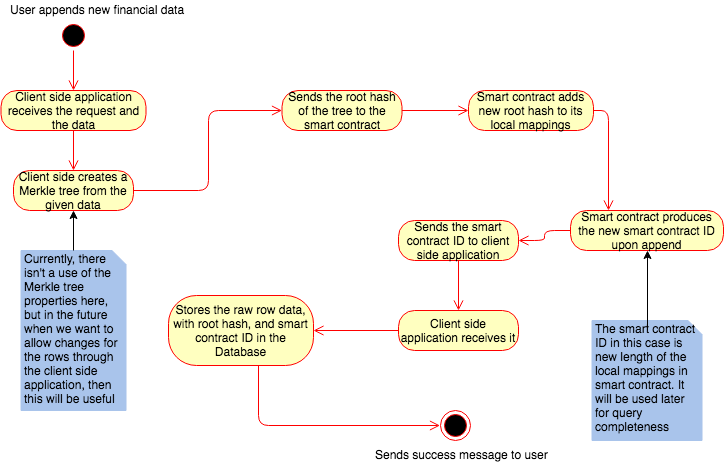
\includegraphics[width=1.0\textwidth]{images/appendRowFinancials.png}
	\caption{\label{fig:appendRowFinancials}Activity diagram of appending a row to the financials record}
\end{figure}

\begin{enumerate}
	\item User appends a new financial data, providing all the required information to be in the database
	\item Client-side application then creates a Merkle tree from the given raw data
	\item Sends the root hash of the created Merkle tree to the smart contract
	\item Smart contract appends that new root hash into its local mappings.
	\item Smart contract increments the new length of the mapping, which is the smart contract ID that is going to be returned. This acts as an identifier to which hash belongs to which financial row. It is also used to preserve the ordering of the hashes which will later be used for query completeness.
	\item Smart contract sends back the smart contract ID to the client-side application
	\item Client-side application saves the raw financial data, with the root hash, and the smart contract ID in the database. (See also Table \ref{table:recordsOffChain} to see how records are saved in the database)
\end{enumerate}

\subparagraph{Query Completeness Steps}
Below shows the implemented step by step actions when a user requests to perform query completeness. Figure \ref{fig:queryCompleteness} shows the activity diagram of the steps described below:

\begin{figure}[h]
	\centering
	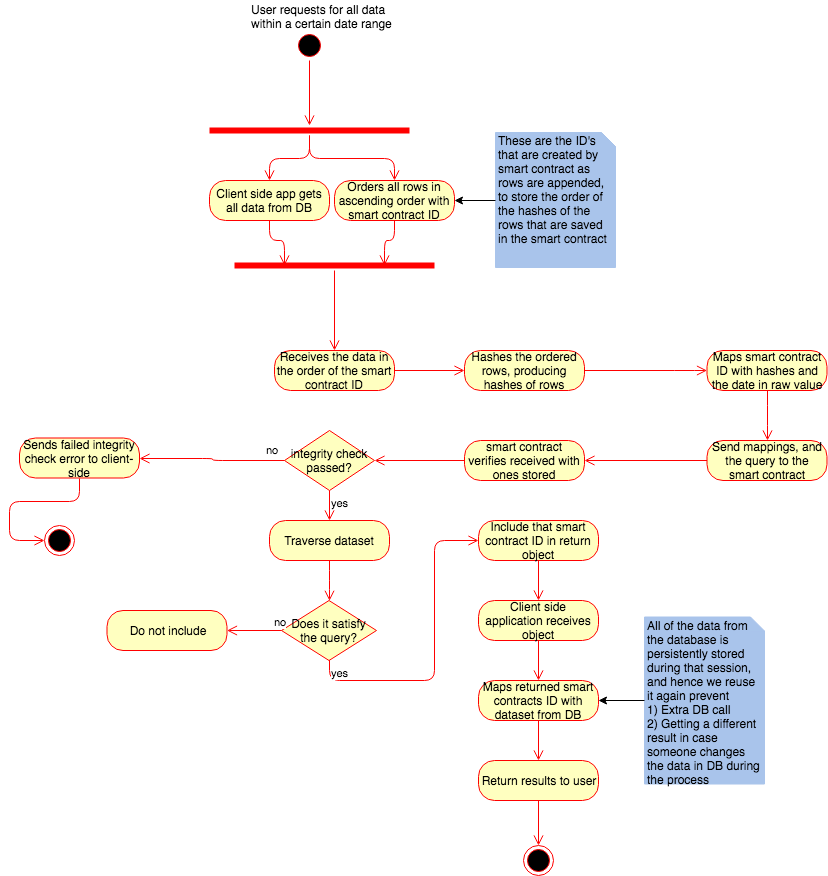
\includegraphics[width=1.0\textwidth]{images/queryCompleteness.png}
	\caption{\label{fig:queryCompleteness}Activity diagram for query completeness}
\end{figure}

\begin{enumerate}
	\item User requests to get all of financial data that are within the date range the user has requested.
	\item The client-side application gets all data from the database in the ascending order of the smart contract ID. This ID is generated by the smart contract to keep the ordering of the hashes that are stored in the smart contract. It is generated upon appending a financial record through the smart contract.
	\item The client-side application hashes each of the rows in the table.
	\item It will then map the hashes of the row and the raw date value to the smart contract ID.
	\item The client-side application sends the mapping with the query to the smart contract.
	\item The smart contract checks if it got the right data, the right amount of rows and the correct table overall by iterating over the provided root hashes and comparing them to the stored hashes in the local mapping.
		\begin{enumerate}
		\item If smart contract cannot verify the rows, then it will throw an integrity check error to the client-side application as an event.
		\item If the smart contract can confirm this, it checks the query condition for every row and returns an array of booleans indicating all the indexes of rows that fulfill the query. Dates are intentionally stored as “uint” to ease the query function in the smart contract. For example 1, March, 2018 -> 20180301
		\end{enumerate}
	\item Smart contract triggers an event to return back all the smart contract IDs that have satisfied the query.
	\item The client-side application listens to this event and returns the specified rows to the user subsequently.
\end{enumerate}
